\newif\ifglobal

%%%%%%%%%%%%%%%%%%%%%%%
%%% Compile to view %%%
%%%%%%%%%%%%%%%%%%%%%%%

%%%%%%%%%%%%%%%%%%%%%%%%%%%%%%%%%%%%%%%%%%%%%%%%%%%
%%% Readme:                                     %%%
%%% https://www.overleaf.com/read/bwdjvfjksvjy/ %%%
%%%%%%%%%%%%%%%%%%%%%%%%%%%%%%%%%%%%%%%%%%%%%%%%%%%

% >>> M?: marks a module setting number or important notice

% >>> M4: Set {./relative-path} to external files for this module <<<
\def \modulefiles {./30-RMT}
% To add an external file, use:
% (Replace '---' with actual filename)
% '\input{\modulefiles/tables/---.tex}' for tables
% '\includegraphics{\modulefiles/figures/---}' for figures
% '\subfile{\modulefiles/---}' for register files


% >>> M1: This module is in global project? <<<
% 'YES' - uncomment; 'NO' - comment out
\globaltrue

\ifglobal
    \documentclass[main\_\_CN.tex]{subfiles}

\else
    % Font "FandolSong-Regular" used by ctex does not have GSUB table.
    % It causes warnings that do not affect compilation and can be ignored.
    \PassOptionsToPackage{quiet}{fontspec}

    \documentclass[openany, 10pt]{book}

    % >>> M2: In ./00-shared/preamble-trm-module, also find
    %         settings for visibility of todo notes, watermark <<<
    \usepackage{preamble-trm-module}

    % Enable Chinese typesetting
    \usepackage{ctex}

    % >>> M3: Temporary labels in Chinese
    %         you can add your own labels there <<<
    \myexternaldocument{./00-shared/temp-labels-cn}

\fi %\ifglobal


\setcounter{secnumdepth}{4}


% >>> M5: If this module needs any updates in
% './00-shared/preamble-trm-module.sty'
% (include additional package, etc.), contact your module PM
% or create the file './00-shared/changelog.tex' make the
% necessary updates yourself and document them in this file <<<

% Make text left-aligned and allow latex to break pages naturally, comment out for full justification
\raggedright
\raggedbottom


\begin{document}


% Sets language into which pre-defined bits of text are translated
\selectlanguage{chinese}
\setchineseformatting


% Do not delete this block
\ifglobal
% Add the following front matter if
% this module is outside of global project
\else
    \InputIfFileExists{readme}{}{}
    \listoftodos
    {\let\clearpage\relax \listofdonetodos}
    \tableofcontents
    %\listoftables
    %\listoffigures
\fi


%%%%%%%%%%%%%%%%%%%%%%%%%
%%% TRM Module Begins %%%
%%%%%%%%%%%%%%%%%%%%%%%%%

\hypertarget{rmt}{}
\chapter{红外遥控 (RMT)}
\label{mod:rmt}

\section{概述}
RMT（红外遥控器）是一个红外发送／接收控制器,其特殊设计支持生成各类信号。红外遥控发射器从内置的 RAM（随机存取存储器）区中读取连续的脉冲码,并对输出信号进行载波调制。接收器检测输入信号,并 进行滤波,然后将信号高低电平以及长度值存入 RAM 中。

RMT 有 8 个通道，编码为 0 \verb+~+ 7，每个通道有一组功能相同的寄存器。为了方便叙述，以 \textcolor{red}{\it{n}} 表示各个通道。

\section{功能描述}
\subsection{RMT 架构}
\begin{figure}[H]
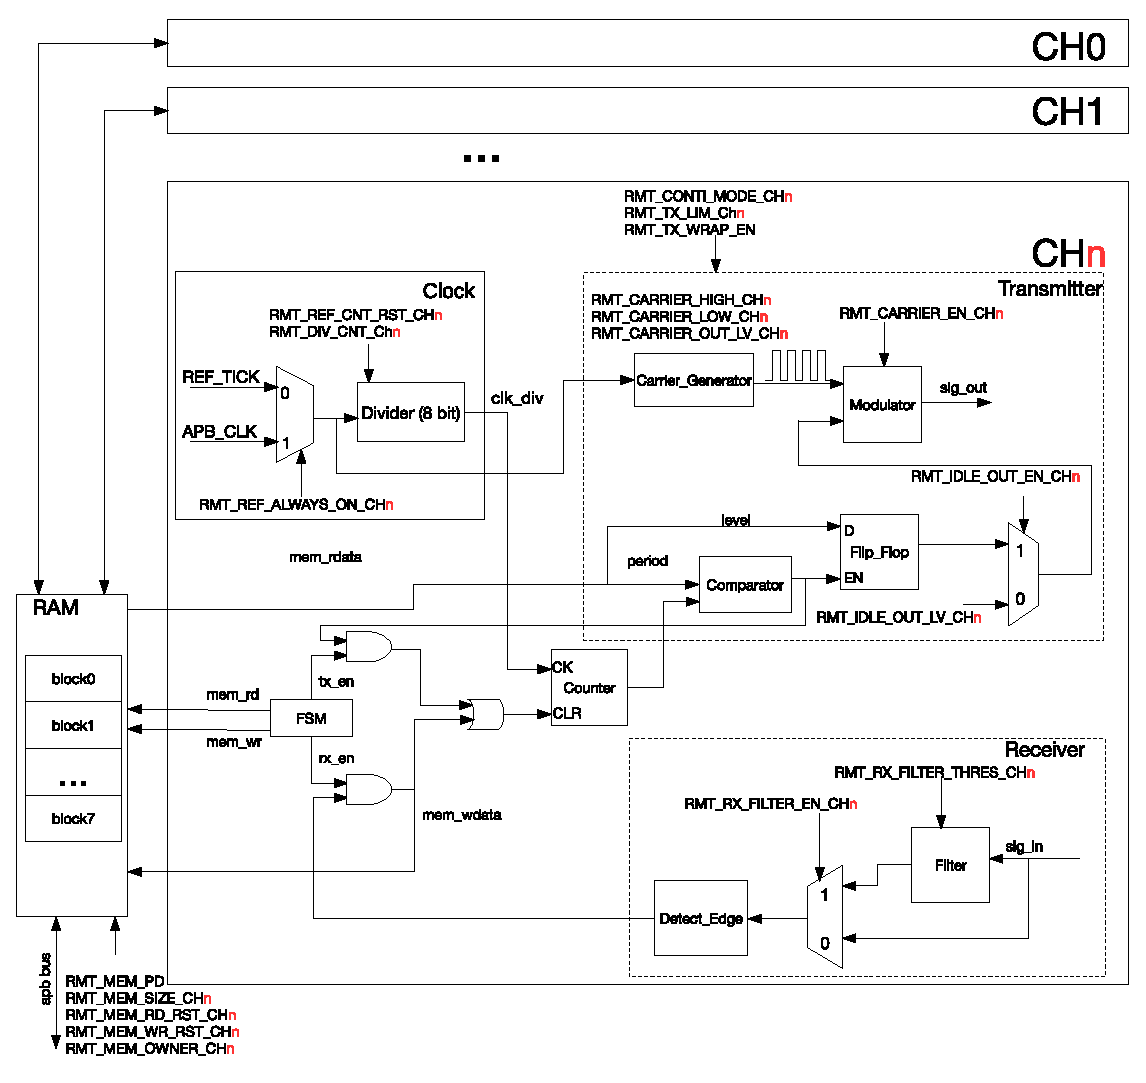
\includegraphics[width=0.7\textwidth]{./30-RMT/figures/rmt2-1_20190313}
\centering
\caption{RMT 架构} \label{Figure:RMT2-1}
\end{figure}

RMT 有 8 个独立通道,每个通道内部有一个发送器和一个接收器,发送和接收不可同时工作。8 个通道共享一块 512x32 bit 的 RAM。RAM 可由处理器内核通过 APB 总线进行读写。发射器可以对信号进行载波调制。软件可以通过配置 RMT\_REF\_ALWAYS\_ON\_CH\textcolor{red}{\it{n}} 选择每个通道的工作时钟：80 MHz APB（外围总线）时钟或者 REF\_TICK。

\subsection{RMT RAM}\label{RMTRAM}
\begin{figure}[htb!]

\includegraphics[width=0.5\textwidth]{./30-RMT/figures/rmt_data_structure}
\centering
\caption{数据结构} \label{Figure:RMT2-2}
\end{figure}
RAM 中数据结构如图 \ref{Figure:RMT2-2} 所示，由低 16 位和高 16 位组成。两个字段中 level 表示电平高低值，period 表示
level 持续的分频时钟（图 \ref{Figure:RMT2-1} 中 clk\_div）周期数。period 为 0 表示结束标志，发射器停止发送数据，接收器在检测到接收的信号变成空闲状态后会写此值。

RAM 可以通过 APB 总线进行访问，其起始地址为 0x3FF56800。每个通道可使用的 RAM 范围按照 64x32 bit 分成 8 个 block。默认情况下每个通道可使用的 block 数量为 1（通道 0 使用 block0，通道 1 使用 block1，以此类推）。当通道 \textcolor{red}{\it{n}} 发送的数据量大于可使用的 block 时，除了可以通过配置 RMT\_MEM\_SIZE\_CH\textcolor{red}{\it{n}} 寄存器扩展 block 还可以进行乒乓操作。将 RMT\_MEM\_SIZE\_CH\textcolor{red}{\it{n}} 寄存器配置为 >1,意味着此通道会占用下一个通道的 block。通道 \textcolor{red}{\it{n}} 使用的 RAM 地址范围为:

$ \textrm{start\_addr\_ch}\textcolor{red}{\it{n}} = \textrm{0x3FF56800} + 64*4*\textcolor{red}{\it{n}}$\textrm{,   and} \\
$ \textrm{end\_addr\_ch}\textcolor{red}{\it{n}} = \textrm{0x3FF56800} + (64*4*\textcolor{red}{\it{n}}+64*4*\textrm{RMT\_MEM\_SIZE\_CH}\textcolor{red}{\it{n}})\textrm{mod}(512*4)-4 $

为了防止数据覆盖，可以通过配置 RMT\_MEM\_OWNER\_CH\textcolor{red}{\it{n}} 来表示发射器或者接收器对于信道 \textcolor{red}{\it{n}} 的 RAM 使用权。当配置不正确时，则会产生 RMT\_CH\textcolor{red}{\it{n}}\_ERR 中断。

{\bfseries 注意：}当开启连续发送模式（即置位 RMT\_REG\_TX\_CONTI\_MODE）时，发送器会连续发送通道中的数据（即从第一个数据发送到最后一个数据，再从第一个发送到最后一个，依此类推）。在连续发送模式下，第 N 次和第 N+1 次之间会有一个 clk\_div 周期的 IDLE 电平。

\subsection{时钟}
软件可以通过配置 RMT\_REF\_ALWAYS\_ON\_CH\textcolor{red}{\it{n}} 选择每个通道的工作时钟：80 MHz APB 时钟或者 REF\_TICK，请参考章节\hyperref[mod:resclk]{复位和时钟}。经过 8 位宽分频器分频之后的时钟供载波发生器以及计数器使用。分频器可以通过配置 RMT\_REF\_CNT\_RST\_CH\textcolor{red}{\it{n}} 进行复位。其分频系数由 RMT\_DIV\_CNT\_CH\textcolor{red}{\it{n}} 控制。

\subsection{发射器}\label{rmt:transmitter}
当 RMT\_TX\_START\_CH\textcolor{red}{\it{n}} 置为 1 时，通道 \textcolor{red}{\it{n}} 的发射器开始从 RAM 中读取数据。发射器每读取一次 RAM，可以获得 32 位的数据,低 16 位首先发送，高 16 位其次发送。

当发送的数据量大于可使用的 block 时,可以进行乒乓操作。在进行乒乓操作前配置 RMT\_TX\_LIM\_CH\textcolor{red}{\it{n}}，当发送的数据量大于等于 RMT\_TX\_LIM\_CH\textcolor{red}{\it{n}} 时，会产生 RMT\_CH\textcolor{red}{\it{n}}\_TX\_THR\_EVENT\_INT 中断，软件可以在检测 到该中断之后更新已发送的数据。当发射器发送的数据量达到 block 的上限时,发射器会返回到 start\_addr\_ch\textcolor{red}{\it{n}} 继续循环发送。

只有当数据中 period 等于 0 时，发射器将结束工作并产生 RMT\_CH\textcolor{red}{\it{n}}\_TX\_END\_INT 中断，然后返回空闲状态。空闲状态默认发送的电平为结束标志 0 对应的电平，此时也可以通过配置 RMT\_IDLE\_OUT\_EN\_CH\textcolor{red}{\it{n}} 和 RMT\_IDLE\_OUT\_LV\_CH\textcolor{red}{\it{n}} 来控制发射器的输出电平。

输出信号可以通过配置 RMT\_CARRIER\_EN\_CH\textcolor{red}{\it{n}} 进行载波调制。载波的频率可以通过 RMT\_CARRIER\_HIGH\_CH\textcolor{red}{\it{n}} 和 RMT\_CARRIER\_LOW\_CH\textcolor{red}{\it{n}} 进行设置。

\subsection{接收器}
当 RMT\_RX\_EN\_CH\textcolor{red}{\it{n}} 置为 1 时，计数器开始测量信号的长度并在下一次信号沿 变化时将上次的信号高低电平以及长度值存入 RAM。当发射器长时间检测不到信号沿变化即计数器的值大于等于 RMT\_IDLE\_THRES\_CH\textcolor{red}{\it{n}} 时，接收器结束接收过程，产生 RMT\_CH\textcolor{red}{\it{n}}\_RX\_END\_INT 中断并返回空闲状态。

输入信号可以通过置位 RMT\_RX\_FILTER\_EN\_CH\textcolor{red}{\it{n}} 来进行滤波。滤波器可以滤除信号宽度小于\\ RMT\_RX\_FILTER\_THRES\_CH\textcolor{red}{\it{n}} 个 APB 时钟周期的脉冲。

当 RMT 模块不工作时，可以通过配置 RMT\_MEM\_PD 寄存器使 RAM 工作于低功耗模式。
\subsection{中断}
\begin{itemize}
\item \label{int:RMTCHnTXTHREVENTINT}RMT\_CH\textcolor{red}{\it{n}}\_TX\_THR\_EVENT\_INT：发射器每发送 RMT\_CH\textcolor{red}{\it{n}}\_TX\_LIM\_REG 的数据，即触发一次此中断。
\item \label{int:RMTCHnTXENDINT}RMT\_CH\textcolor{red}{\it{n}}\_TX\_END\_INT：当发射器停止发送信号时,即触发此中断。
\item \label{int:RMTCHnRXENDINT}RMT\_CH\textcolor{red}{\it{n}}\_RX\_END\_INT：当接收器停止接收信号时,即触发此中断。
\end{itemize}

\hypertarget{rmt-reg-summ}{}
\section{寄存器列表}\label{sec:rmt-reg-summ}

本小节的所有地址均为相对于 RMT 基地址的地址偏移量（相对地址），具体基地址请见章节 \ref{mod:sysmem} \textit{\nameref{mod:sysmem}} 中的表 \ref{table:Peripheral_Address_Mapping}。

请查看章节 \hyperref[glossary-access-types]{\textit{寄存器的访问类型}}，了解“访问”列缩写的含义。

\subfile{\modulefiles/rmt-reg_summary_cn.tex}

\section{寄存器}

本小节的所有地址均为相对于 RMT 基地址的地址偏移量（相对地址），具体基地址请见章节 \ref{mod:sysmem} \textit{\nameref{mod:sysmem}} 中的表 \ref{table:Peripheral_Address_Mapping}。寄存器绝对地址见章节 \ref{sec:rmt-reg-summ} \textit{\nameref{sec:rmt-reg-summ}}。

关于保留 (reserved) 域的处理，请查看章节 \hyperref[programming-reserved-field]{\textit{如何配置寄存器的保留域}}。

\subfile{\modulefiles/rmt-reg_cn.tex}

\end{document}
